\begin{frame}{‌مسئله انتخاب فعالیت‌ها}
\begin{itemize}\itemr
\item[-]
در مسئله انتخاب فعالیت‌ها
\fn{1}{activity selection problem}
، تعدادی فعالیت به طور همزمان می‌خواهند انجام شوند به طوری‌که این فعالیت‌ها از یک منبع مشترک استفاده می‌کنند و این منبع مشترک نمی‌تواند به طور همزمان توسط فعالیت‌ها استفاده شود. می‌خواهیم مجموعه‌ای از فعالیت‌ها را انتخاب کنیم، به طوری که بیشترین تعداد فعالیت‌ها بتوانند اجرا شوند.
\item[-]
فرض کنید شما مسئول زمانبندی یک اتاق کنفرانس هستید. به شما مجموعهٔ
\m{S = \{a_1,a_2, \cdots, a_n \}}
شامل n فعالیت داده شده است که می‌خواهند اتاق کنفرانس را رزرو کنند. در این اتاق در یک زمان تنها یک فعالیت می‌تواند صورت بگیرد.
\end{itemize}
\end{frame}


\begin{frame}{‌مسئله انتخاب فعالیت‌ها}
\begin{itemize}\itemr
\item[-]
هر فعالیت
\m{a_i}
یک زمان شروع
\fn{1}{state time}
\m{s_i}
و یک زمان پایان
\fn{2}{finish time}
\m{f_i}
دارد به طوری‌که
\m{0 \leqslant s_i < f_i < \infty}.
اگر فعالیت
\m{a_i}
انتخاب شود، آنگاه این فعالیت می‌تواند در بازهٔ زمانی
\m{[s_i,f_i)}
انجام شود. دو فعالیت
\m{a_i}
و
\m{a_j}
سازگار
\fn{3}{compatible}
گفته می‌شوند اگر بازه‌های زمانی
\m{[s_i,f_i)}
و
\m{[s_j,f_j)}
تداخل نداشته باشند. دو فعالیت تداخل ندارند اگر
\m{s_i \geqslant f_j}
یا
\m{s_j \geqslant f_i}
. در مسئلهٔ انتخاب فعالیت‌ها، هدف این است که بیشترین تعداد فعالیت‌های سازگار از یک مجموعهٔ فعالیت‌ها انتخاب شوند.
\item[-]
فرض می‌کنیم فعالیت‌ها بر اساس زمان پایان‌شان مرتب شده‌اند. به عبارت دیگر :
\begin{align*}
\m{f_1 \leqslant f_2 \leqslant f_3 \leqslant \cdots \leqslant f_{n-1} \leqslant f_n}
\end{align*}
\end{itemize}
\end{frame}


\begin{frame}{‌مسئله انتخاب فعالیت‌ها}
\begin{itemize}\itemr
\item[-]
برای مثال مجموعه‌ای از فعالیت‌ها در جدول زیر را در نظر بگیرید.
\begin{figure}
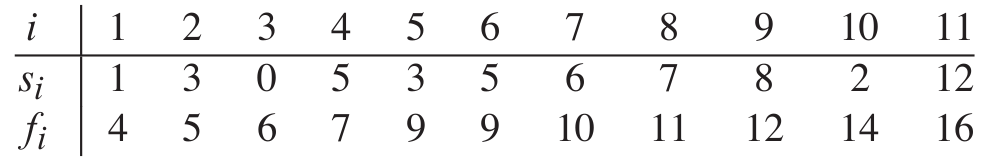
\includegraphics[width=0.7\textwidth]{figs/chap05/activity-example}
\end{figure}
\item[-]
مجموعهٔ
\m{\{a_3,a_9,a_{11}\}}
مجموعه‌ای از فعالیت‌های سازگار است ولی بزرگ‌ترین مجموعهٔ فعالیت‌های سازگار نیست چراکه
\m{\{a_1,a_4,a_8,a_{11}\}}
تعداد بیشتری فعالیت را شامل می‌شود.
همچنین مجموعهٔ
\m{\{a_2,a_4,a_9,a_{11}\}}
تعداد چهار فعالیت را شامل می‌شود.
\end{itemize}
\end{frame}



\begin{frame}{‌مسئله انتخاب فعالیت‌ها}
\begin{itemize}\itemr
\item[-]
در اینجا ابتدا سعی می‌کنیم مسئلهٔ انتخاب فعالیت‌ها را توسط برنامه‌ریزی پویا حل کنیم.
\item[-]
 فرض کنید
\m{S_{ij}}
مجموعه‌ای از فعالیت‌ها باشد که پس از اتمام فعالیت
\m{a_i}
آغاز
و قبل از شروع فعالیت
\m{a_j}
تمام می‌شوند.
فرض کنید می‌خواهیم حداکثر فعالیت‌های سازگار
\m{S_{ij}}
را پیدا کنیم و فرض کنید
\m{A_{ij}}
مجموعه‌ای است که شامل حداکثر تعداد فعالیت‌های سازگار از مجموعهٔ
\m{S_{ij}}
است.
\item[-]
حال فرض کنید
\m{a_k}
یکی از فعالیت‌ها در مجموعهٔ
\m{A_{ij}}
است. در اینجا دو زیر مسئله داریم : مسئلهٔ یافتن حداکثر فعالیت‌های سازگار در
\m{S_{ik}}
(که شامل فعالیت‌هایی می‌شود که پس از اتمام
\m{a_i}
آغاز
و قبل از شروع
\m{a_k}
پایان می‌یابند) و مسئلهٔ یافتن حداکثر فعالیت‌های سازگار در
\m{S_{kj}}
(که شامل فعالیت‌هایی می‌شود که پس از اتمام
\m{a_k}
آغاز
و قبل از شروع
\m{a_j}
پایان می‌یابند).
\end{itemize}
\end{frame}

\begin{frame}{‌مسئله انتخاب فعالیت‌ها}
\begin{itemize}\itemr
\item[-]
در گام اول باید ثابت کنیم مسئله دارای زیرساختار بهینه است.
\item[-]
 فرض کنید
\m{a_k}
در مجموعهٔ جواب
\m{A_{ij}}
است.
حال فرض کنید
\m{A_{ik} = A_{ij}\cap S_{ik}}
و
\m{A_{kj} = A_{ij}\cap S_{kj}},
بنابراین
\m{A_{ik}}
شامل فعالیت‌هایی در
\m{A_{ij}}
می‌شود که قبل از شروع
\m{a_k}
پایان می‌یابند و
\m{A_{kj}}
شامل فعالیت‌هایی در
\m{A_{ij}}
می‌شود که پس از اتمام
\m{a_k}
شروع می‌شوند.
\item[-]
اگر
\m{a_k}
در 
\m{A_{ij}}
باشد، الزاما
\m{A_{ik}}
جواب مسئله
\m{S_{ik}}
و
\m{A_{kj}}
جواب مسئله
\m{S_{kj}}
است.
\item[-]
با استفاده از برهان خلف می‌توانیم اثبات کنیم پاسخ بهینه برای
\m{S_{ij}}
شامل پاسخ بهینه برای دو زیر مسئله
\m{S_{ik}}
و
\m{S_{kj}}
می‌شود. اگر می‌توانستیم مجموعه
\m{A'_{kj}}
از حداکثر فعالیت‌های سازگار
\m{S_{kj}}
را پیدا کنیم به طوری‌که
\m{|A'_{kj}| > |A_{kj}|}
آنگاه می‌توانستیم از
\m{A'_{kj}}
به جای
\m{A_{kj}}
در زیر مسئلهٔ
\m{S_{ij}}
استفاده کنیم و بنابراین داشتیم :\\
\m{|A_{ik}| + |A'_{kj}| + 1 > |A_{ik}| + |A_{kj}| + 1 = |A_{ij}|}
که با فرض اینکه
\m{A_{ij}}
جواب بهینه است در تناقض است.
\end{itemize}
\end{frame}

\begin{frame}{‌مسئله انتخاب فعالیت‌ها}
\begin{itemize}\itemr
\item[-]
طبق تعریف می‌دانیم
حداکثر تعداد فعالیت‌ها در 
\m{S_{ik}}
برابر است با
\m{A_{ik}}
و
حداکثر تعداد فعالیت‌ها در 
\m{S_{kj}}
برابر است با
\m{A_{kj}} .
\item[-]
بنابراین داریم
\m{A_{ij} = A_{ik}\cup \{a_k \} \cup A_{kj}}
و در نتیجه
\m{|A_{ij}| = |A_{ik}| + |A_{kj}| + 1}.
\end{itemize}
\end{frame}


\begin{frame}{‌مسئله انتخاب فعالیت‌ها}
\begin{itemize}\itemr
\item[-]
فرض کنید اندازه مجموعه جواب بهینه برای
\m{S_{ij}}
را با
\m{c[i,j]}
نشان دهیم، 
بنابراین 
\m{|A_{ij}| = c[i,j]} .
\item[-]
آنگاه می توانیم بنویسیم :
\m{c[i,j] = c[i,k] + c[k,j] + 1}.
\item[-]
از آنجایی که نمی‌دانیم به ازای کدام
\m{a_k}
جواب بهینه به‌دست می‌آید، بنابراین باید همهٔ
\m{a_k}
ها را در نظر بگیریم تا جواب بهینه را به دست آوریم.
\begin{align*}
\m{c[i,j] = } \left\{ \begin{array}{lr}
					\m{0} & \m{S_{ij} = \emptyset}~~\text{اگر}\\
					\m{\max \{c[i,k] + c[k,j] + 1 : a_k \in S_{ij} \}} & \m{S_{ij} \neq \emptyset}~~\text{اگر}
					\end{array}\right.
\end{align*}
\item[-]
سپس می‌توانیم این مسئله را به روش برنامه‌ریزی پویا حل کنیم.
%\item[-]
%مشاهده خواهیم کرد که به جای چند انتخاب برای زیر مسئله‌های بهینه، در این مسئله همیشه در هنگام استفاده از برنامه‌ریزی پویا، تنها یک زیرمسئلهٔ بهینه وجود دارد. انتخاب این زیرمسئلهٔ بهینه همان انتخاب حریصانه است. درواقع با یک انتخاب حریصانه در هرگام از الگوریتم در نهایت به جواب بهینه دست پیدا می‌کنیم.
\end{itemize}
\end{frame}


\begin{frame}{‌مسئله انتخاب فعالیت‌ها}
\begin{itemize}\itemr
\item[-]
می‌توانیم رابطهٔ به دست آمده را ساده‌تر کنیم.
\item[-]
در مجموعهٔ
\m{S_{ij}}
همیشه یکی از عناصر به عنوان اولین عنصری است که در مجموعهٔ
\m{A_{ij}}
قرار می‌گیرد.
\item[-]
می‌خواهیم اولین عنصر از مجموعهٔ 
\m{S_{ij}}
که در مجموعهٔ 
\m{A_{ij}}
قرار می‌گیرد را انتخاب کنیم.
\item[-]
پس صورت مسئله را تغییر می‌دهیم.
\end{itemize}
\end{frame}


\begin{frame}{‌مسئله انتخاب فعالیت‌ها}
\begin{itemize}\itemr
\item[-]
فرض کنید
\m{S_k = \{a_i  \in S : s_i \geqslant f_k \}}
مجموعه‌ای از فعالیت‌ها باشد که پس از اتمام
\m{a_k}
آغاز می‌شوند.
\item[-]
اولین فعالیت در 
\m{S_k}
که در بزرگترین مجموعهٔ سازگار فعالیت‌ها قرار می‌گیرد کدام است؟
\end{itemize}
\end{frame}

\iffalse
\begin{frame}{‌مسئله انتخاب فعالیت‌ها}
\begin{itemize}\itemr
\item[-]
انتخاب حریصانه
\m{a_1}
اولین فعالیتی است که
انتخاب می‌شود و پس از آن
\m{S_1}
زیر مسئلهٔ بعدی است که باید حل شود.
\item[-]
بنابراین اگر
\m{a_1}
متعلق به مجموعهٔ جواب بهینه باشد، آنگاه مجموعه جواب بهینه برای کل مسئله برابر است با
\m{a_1}
 و تمام فعالیت‌هایی که به جواب زیر مسئلهٔ
\m{S_1}
تعلق دارند.
\item[-]
این راه‌حل را به طور شهودی به دست آوردیم. حال باید اثبات کنیم که این راه‌حل درست است.
\end{itemize}
\end{frame}
\fi

\begin{frame}{‌مسئله انتخاب فعالیت‌ها}
\begin{itemize}\itemr
\item[-]
قضیه : فرض کنید
\m{S_k}
مجموعه‌ای غیر تهی از فعالیت‌هاست و
\m{a_m}
فعالیتی است در
\m{S_k}
که کوچک‌ترین زمان پایان را دارد. آنگاه
\m{a_m}
در بزرگ‌ترین مجموعهٔ فعالیت‌های سازگار
\m{S_k}
قرار دارد.
\item[-]
اثبات : فرض کنید
\m{A_k}
بزرگ‌ترین مجموعهٔ فعالیت‌های سازگار
\m{S_k}
باشد و
\m{a_j}
فعالیتی در
\m{A_k}
باشد که کوچکترین زمان پایان را دارد. اگر
\m{a_j = a_m}
باشد به نتیجه مطلوب رسیده‌ایم یعنی در واقع
\m{a_m}
متعلق به بزرگ‌ترین مجموعهٔ فعالیت‌های سازگار
\m{S_k}
است.
\item[-]
حال فرض کنیم
\m{a_j \neq a_m}
باشد. مجموعهٔ
\m{A'_k = (A_k - \{a_j\}) \cup \{a_m\}}
را به عنوان مجموعه‌ای که شامل
\m{a_j}
نیست ولی
\m{a_m}
را شامل می‌شود در نظر بگیرید. فعالیت‌های
\m{A'_k}
سازگار هستند، زیرا فعالیت‌های
\m{A_k}
سازگار هستند،
و
\m{a_j}
اولین فعالیت در
\m{A_k}
است که به اتمام می‌رسد و
\m{f_m \leqslant f_j}.
از آنجایی که
\m{|A'_k| = |A_k|}
، نتیجه می‌گیریم که
\m{A'_k}
نیز بزرگ‌ترین مجموعه فعالیت‌های سازگار
\m{S_k}
است که
\m{a_m}
را نیز شامل می‌شود.
\end{itemize}
\end{frame}



\begin{frame}{‌مسئله انتخاب فعالیت‌ها}
\begin{itemize}\itemr
\item[-]
فرض کنید اندازه مجموعه جواب بهینه برای
\m{S_{k}}
را با
\m{c[k]}
نشان دهیم، 
بنابراین 
\m{|A_{k}| = c[k]} .
\item[-]
اگر اولین عضو مجموعهٔ
\m{S_k}
فعالیت
\m{a_m}
باشد، طبق قضیه قبل
\m{a_m}
در
\m{A_k}
است.
  مجموعه فعالیت‌های باقیمانده
\m{S_{m}}
است و در اینصورت
می توانیم بنویسیم :
\m{c[k] = 1 + c[m]}.
\item[-]
بنابراین می‌توانیم بنویسیم:
\begin{align*}
\m{c[k] = } \left\{ \begin{array}{lr}
					\m{0} & \m{S_{k} = \emptyset}~~\text{اگر}\\
					\m{1 + c[m]} & \text{باشد.}~\m{S_k}~\text{اولین عضو}~\m{a_m}~\text{و}~\m{S_{k} \neq \emptyset}~~\text{اگر}
					\end{array}\right.
\end{align*}
\item[-]
در اینجا یک رابطهٔ بازگشتی به دست آوردیم که همیشه تنها یک انتخاب بهینه در آن وجود دارد.
در صورتی که بتوانیم چنین رابطهٔ بازگشتی برای یک مسئله پیدا کنیم، که در آن همیشه یک انتخاب بهینه وجود داشته باشد، می‌توانیم مسئله را با استفاده از روش حریصانه حل کنیم.
%\item[-]
%مشاهده خواهیم کرد که به جای چند انتخاب برای زیر مسئله‌های بهینه، در این مسئله همیشه در هنگام استفاده از برنامه‌ریزی پویا، تنها یک زیرمسئلهٔ بهینه وجود دارد. انتخاب این زیرمسئلهٔ بهینه همان انتخاب حریصانه است. درواقع با یک انتخاب حریصانه در هرگام از الگوریتم در نهایت به جواب بهینه دست پیدا می‌کنیم.
\end{itemize}
\end{frame}


\iffalse
\begin{frame}{‌مسئله انتخاب فعالیت‌ها}
\begin{itemize}\itemr
\item[-]
اما این مسئله را می‌توانیم به روشی ساده‌تر نیز حل کنیم. به طور شهودی می‌توانیم حدس بزنیم که باید فعالیت‌هایی را انتخاب کنیم که امکان انتخاب حداکثر تعداد فعالیت‌ها را به ما بدهند، بنابراین به طور شهودی می‌توانیم حدس بزنیم باید فعالیتی ابتدا تمام شود که زمان پایان آن زودتر باشد تا تعداد بیشتری فعالیت بتوانند به عنوان فعالیت بعدی انتخاب شوند.
\item[-]
به عبارت دیگر از آنجایی که فعالیت‌ها به ترتیب بر اساس زمان پایان‌شان مرتب شده‌اند و در ابتدا فعالیتی انتخاب می‌شود که زمان پایان آن از همه زودتر باشد، بنابراین فعالیت
\m{a_1}
انتخاب می‌شود. سپس فعالیتی انتخاب شود که زمان شروع آن پس از زمان اتمام
\m{a_1}
باشد تا با
\m{a_1}
تداخل نداشته باشد و ضمنا زمان پایان آن از بقیه فعالیت‌های ممکن کمتر باشد. پس اولین فعالیت پس از
\m{a_1}
که زمان شروع آن پس از اتمام
\m{a_1}
است انتخاب می‌شود.
\end{itemize}
\end{frame}
\fi

\iffalse
\begin{frame}{‌مسئله انتخاب فعالیت‌ها}
\begin{itemize}\itemr
\item[-]
گرچه توانستیم مسئله انتخاب فعالیت‌ها را با استفاده از برنامه‌ریزی پویا حل کنیم، ولی با استفاده از قضیه قبل می‌توانیم این مسئله را به روشی دیگر نیز حل کنیم.
\end{itemize}
\end{frame}
\fi


\begin{frame}{‌مسئله انتخاب فعالیت‌ها}
\begin{itemize}\itemr
\item[-]
بنابراین در هر بار باید فعالیتی را انتخاب کنیم که زمان پایان آن از همهٔ فعالیت‌های دیگر کوچک‌تر باشد. سپس تنها فعالیت‌هایی را نگه‌داریم که زمان شروع آنها از زمان پایان فعالیت انتخاب شده بزرگ‌تر است و فرایند را تکرار کنیم تا جایی که دیگر فعالیتی برای انتخاب نداشته باشیم.
\item[-]
برای حل این مسئله می توانیم از یک الگوریتم بازگشتی استفاده کنیم.
\item[-]
این الگوریتم یک الگوریتم حریصانه است، زیرا در هر مرحله به طور حریصانه فعالیتی انتخاب می‌شود که منجر به تعداد بیشتری فعالیت سازگار شود و در پایان برای مسئلهٔ کلی جواب بهینه پس از حل زیر مسئله ها به صورت بهینه به‌دست می‌آید.
\end{itemize}
\end{frame}



\begin{frame}{‌مسئله انتخاب فعالیت‌ها}
\begin{itemize}\itemr
\item[-]
الگوریتم‌های حریصانه برخلاف الگوریتم‌های برنامه‌ریزی پویا، به صورت از بالا به پایین
\fn{1}{top-down}
انجام می‌شوند.
در روش حریصانه برای حل یک مسئله یک انتخاب حریصانه انجام می‌گیرد، و در گام بعدی مسئله برای زیرمسئلهٔ به دست آمده حل می‌شود.
بنابراین الگوریتم از حل مسئلهٔ اصلی شروع می‌کند و سپس زیرمسئله‌ها را به ترتیب حل می‌کند.
در روش برنامه‌ریزی پویا ابتدا زیرمسئله‌ها حل می‌شوند تا در پایان جواب مسئلهٔ اصلی به دست آید، پس این الگوریتم‌ها به صورت از پایین به بالا
\fn{2}{bottom-up}
انجام می‌شوند.
\end{itemize}
\end{frame}


\begin{frame}{‌مسئله انتخاب فعالیت‌ها}
\begin{itemize}\itemr
\item[-]
در الگوریتم زیر، مسئله انتخاب فعالیت توسط حریصانه حل می‌شود. 
\begin{algorithm}[H]\alglr
  \caption{Recursive-Activity-Selector} 
  \begin{algorithmic}[1]
   \Func{Recursive-Activity-Selector}{s, f, k, n}
   \State m = k + 1
   \While{m < = n and s[m] < f[k]} \LeftComment{find the first activity in S[k] to finish}
   		\State m = m + 1
   	\EndWhile
   	\If{m < = n}
   			\State \Return \{a[m]\} $\cup$ Recursive-Activity-Selector (s, f, m, n)
   		\Else
   		    \State \Return $\emptyset$
    \EndIf                   
  \end{algorithmic}
  \label{alg:merge}
\end{algorithm}
\item[-]
برای شروع فرض کنید فعالیت 
\m{a_0}
با زمان اتمام
\m{f_0 = 0}
در مجموعهٔ
\m{S_0 = S}
 وجود دارد. برای شروع، تابع
\texttt{Recursive-Activity-Selector(s,f,0,n)}
فراخوانی می‌شود.
\end{itemize}
\end{frame}


\begin{frame}{‌مسئله انتخاب فعالیت‌ها}
\begin{itemize}\itemr
\item[-]
با فرض اینکه فعالیت‌ها مرتب شده باشند، این الگوریتم در زمان
\ath{n}
مسئله را حل می‌کند.
\end{itemize}
\end{frame}


\begin{frame}{‌مسئله انتخاب فعالیت‌ها}
\begin{itemize}\itemr
\item[-]
یک نمونه از مسئلهٔ انتخاب فعالیت را به صورت زیر در نظر بگیرید.
\begin{figure}
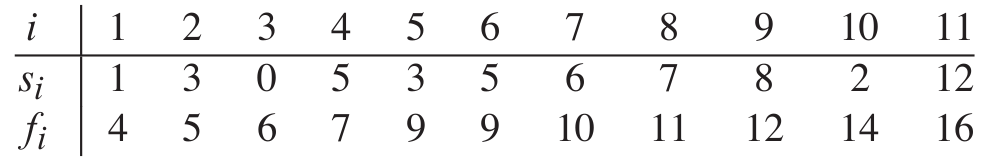
\includegraphics[width=0.7\textwidth]{figs/chap05/activity-example}
\end{figure}
\end{itemize}
\end{frame}

\begin{frame}{‌مسئله انتخاب فعالیت‌ها}
\begin{itemize}\itemr
\item[-]
در مثال زیر این نمونه از مسئله انتخاب فعالیت توسط الگوریتم حریصانه بازگشتی حل شده است.
\begin{figure}
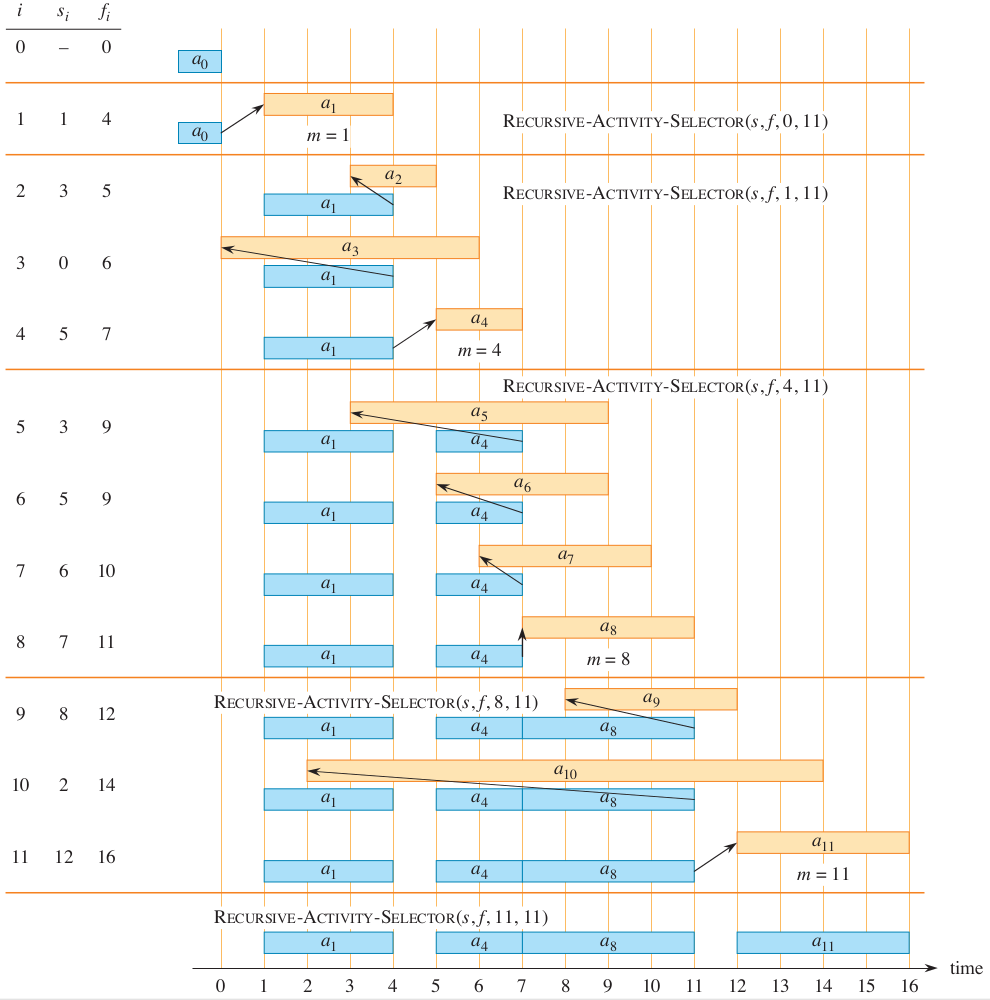
\includegraphics[width=0.47\textwidth]{figs/chap05/activity-recursive-example}
\end{figure}
\end{itemize}
\end{frame}


\iffalse
\begin{frame}{‌مسئله انتخاب فعالیت‌ها}
\begin{itemize}\itemr
\item[-]
این الگوریتم بازگشتی را می‌توانیم به یک الگوریتم غیربازگشتی با یک حلقه تکرار تبدیل کنیم.
\item[-]
به طور کلی همهٔ الگوریتم‌هایی که با یک فراخوانی بازگشتی پایان می‌یابند می‌توانند به الگوریتم‌های غیر بازگشتی با حلقه تکرار تبدیل شوند.
\end{itemize}
\end{frame}
\fi

\begin{frame}{‌مسئله انتخاب فعالیت‌ها}
\begin{itemize}\itemr
\item[-]
الگوریتم زیر مسئله انتخاب فعالیت را به صورت غیر بازگشتی حل می‌کند.
\begin{algorithm}[H]\alglr
  \caption{Greedy-Activity-Selector} 
  \begin{algorithmic}[1]
   \Func{Greedy-Activity-Selector}{s, f, n}
   \State A = \{a[1]\}
   \State k = 1
   \For{m = 2 \To n}
   		\If{s[m] >= f[k]} \LeftComment{is a[m] in S[k] ?}
   				\State A = A $\cup$ \{a[m]\} \LeftComment{yes, so choose it}
   				\State k = m \LeftComment{and continue from there}
   		\EndIf
   	\EndFor
    \State \Return A                       
  \end{algorithmic}
  \label{alg:merge}
\end{algorithm}
\end{itemize}
\end{frame}
